\documentclass[twoside]{book}

% Packages required by doxygen
\usepackage{fixltx2e}
\usepackage{calc}
\usepackage{doxygen}
\usepackage[export]{adjustbox} % also loads graphicx
\usepackage{graphicx}
\usepackage[utf8]{inputenc}
\usepackage{makeidx}
\usepackage{multicol}
\usepackage{multirow}
\PassOptionsToPackage{warn}{textcomp}
\usepackage{textcomp}
\usepackage[nointegrals]{wasysym}
\usepackage[table]{xcolor}

% Font selection
\usepackage[T1]{fontenc}
\usepackage[scaled=.90]{helvet}
\usepackage{courier}
\usepackage{amssymb}
\usepackage{sectsty}
\renewcommand{\familydefault}{\sfdefault}
\allsectionsfont{%
  \fontseries{bc}\selectfont%
  \color{darkgray}%
}
\renewcommand{\DoxyLabelFont}{%
  \fontseries{bc}\selectfont%
  \color{darkgray}%
}
\newcommand{\+}{\discretionary{\mbox{\scriptsize$\hookleftarrow$}}{}{}}

% Page & text layout
\usepackage{geometry}
\geometry{%
  a4paper,%
  top=2.5cm,%
  bottom=2.5cm,%
  left=2.5cm,%
  right=2.5cm%
}
\tolerance=750
\hfuzz=15pt
\hbadness=750
\setlength{\emergencystretch}{15pt}
\setlength{\parindent}{0cm}
\setlength{\parskip}{3ex plus 2ex minus 2ex}
\makeatletter
\renewcommand{\paragraph}{%
  \@startsection{paragraph}{4}{0ex}{-1.0ex}{1.0ex}{%
    \normalfont\normalsize\bfseries\SS@parafont%
  }%
}
\renewcommand{\subparagraph}{%
  \@startsection{subparagraph}{5}{0ex}{-1.0ex}{1.0ex}{%
    \normalfont\normalsize\bfseries\SS@subparafont%
  }%
}
\makeatother

% Headers & footers
\usepackage{fancyhdr}
\pagestyle{fancyplain}
\fancyhead[LE]{\fancyplain{}{\bfseries\thepage}}
\fancyhead[CE]{\fancyplain{}{}}
\fancyhead[RE]{\fancyplain{}{\bfseries\leftmark}}
\fancyhead[LO]{\fancyplain{}{\bfseries\rightmark}}
\fancyhead[CO]{\fancyplain{}{}}
\fancyhead[RO]{\fancyplain{}{\bfseries\thepage}}
\fancyfoot[LE]{\fancyplain{}{}}
\fancyfoot[CE]{\fancyplain{}{}}
\fancyfoot[RE]{\fancyplain{}{\bfseries\scriptsize Generated by Doxygen }}
\fancyfoot[LO]{\fancyplain{}{\bfseries\scriptsize Generated by Doxygen }}
\fancyfoot[CO]{\fancyplain{}{}}
\fancyfoot[RO]{\fancyplain{}{}}
\renewcommand{\footrulewidth}{0.4pt}
\renewcommand{\chaptermark}[1]{%
  \markboth{#1}{}%
}
\renewcommand{\sectionmark}[1]{%
  \markright{\thesection\ #1}%
}

% Indices & bibliography
\usepackage{natbib}
\usepackage[titles]{tocloft}
\setcounter{tocdepth}{3}
\setcounter{secnumdepth}{5}
\makeindex

% Hyperlinks (required, but should be loaded last)
\usepackage{ifpdf}
\ifpdf
  \usepackage[pdftex,pagebackref=true]{hyperref}
\else
  \usepackage[ps2pdf,pagebackref=true]{hyperref}
\fi
\hypersetup{%
  colorlinks=true,%
  linkcolor=blue,%
  citecolor=blue,%
  unicode%
}

% Custom commands
\newcommand{\clearemptydoublepage}{%
  \newpage{\pagestyle{empty}\cleardoublepage}%
}

\usepackage{caption}
\captionsetup{labelsep=space,justification=centering,font={bf},singlelinecheck=off,skip=4pt,position=top}

%===== C O N T E N T S =====

\begin{document}

% Titlepage & ToC
\hypersetup{pageanchor=false,
             bookmarksnumbered=true,
             pdfencoding=unicode
            }
\pagenumbering{alph}
\begin{titlepage}
\vspace*{7cm}
\begin{center}%
{\Large My Project \\[1ex]\large 1 }\\
\vspace*{1cm}
{\large Generated by Doxygen 1.8.13}\\
\end{center}
\end{titlepage}
\clearemptydoublepage
\pagenumbering{roman}
\tableofcontents
\clearemptydoublepage
\pagenumbering{arabic}
\hypersetup{pageanchor=true}

%--- Begin generated contents ---
\chapter{Class Index}
\section{Class List}
Here are the classes, structs, unions and interfaces with brief descriptions\+:\begin{DoxyCompactList}
\item\contentsline{section}{\hyperlink{class_a_v_l_tree}{A\+V\+L\+Tree} \\*Class for A\+VL Tree }{\pageref{class_a_v_l_tree}}{}
\item\contentsline{section}{\hyperlink{structnode}{node} }{\pageref{structnode}}{}
\item\contentsline{section}{\hyperlink{class_node}{Node} }{\pageref{class_node}}{}
\item\contentsline{section}{\hyperlink{struct_r_b_t_node}{R\+B\+T\+Node} \\*\hyperlink{struct_r_b_t_node}{R\+B\+T\+Node} for red black tree }{\pageref{struct_r_b_t_node}}{}
\item\contentsline{section}{\hyperlink{class_r_b_tree}{R\+B\+Tree} \\*Class to represent Red-\/\+Black Tree }{\pageref{class_r_b_tree}}{}
\end{DoxyCompactList}

\chapter{File Index}
\section{File List}
Here is a list of all files with brief descriptions\+:\begin{DoxyCompactList}
\item\contentsline{section}{/home/kavya/\+Desktop/csn261\+\_\+lab\+\_\+assignment1/q1/code/\hyperlink{q1_8c}{q1.\+c} }{\pageref{q1_8c}}{}
\end{DoxyCompactList}

\chapter{Class Documentation}
\hypertarget{struct_node}{}\section{Node Struct Reference}
\label{struct_node}\index{Node@{Node}}
\subsection*{Public Attributes}
\begin{DoxyCompactItemize}
\item 
int \hyperlink{struct_node_a2fdf3febffa37539c09d0a282525033a}{a}
\item 
int \hyperlink{struct_node_a26cb9e26541900f36489bf503338ce4e}{b} \mbox{[}100\mbox{]}
\item 
int \hyperlink{struct_node_acc103d220defd2fdb5aac8e3b03424c6}{size} = 0
\end{DoxyCompactItemize}


\subsection{Detailed Description}


Definition at line 7 of file q1.\+cpp.



\subsection{Member Data Documentation}
\mbox{\Hypertarget{struct_node_a2fdf3febffa37539c09d0a282525033a}\label{struct_node_a2fdf3febffa37539c09d0a282525033a}} 
\index{Node@{Node}!a@{a}}
\index{a@{a}!Node@{Node}}
\subsubsection{\texorpdfstring{a}{a}}
{\footnotesize\ttfamily int Node\+::a}



Definition at line 9 of file q1.\+cpp.

\mbox{\Hypertarget{struct_node_a26cb9e26541900f36489bf503338ce4e}\label{struct_node_a26cb9e26541900f36489bf503338ce4e}} 
\index{Node@{Node}!b@{b}}
\index{b@{b}!Node@{Node}}
\subsubsection{\texorpdfstring{b}{b}}
{\footnotesize\ttfamily int Node\+::b\mbox{[}100\mbox{]}}



Definition at line 10 of file q1.\+cpp.

\mbox{\Hypertarget{struct_node_acc103d220defd2fdb5aac8e3b03424c6}\label{struct_node_acc103d220defd2fdb5aac8e3b03424c6}} 
\index{Node@{Node}!size@{size}}
\index{size@{size}!Node@{Node}}
\subsubsection{\texorpdfstring{size}{size}}
{\footnotesize\ttfamily int Node\+::size = 0}



Definition at line 11 of file q1.\+cpp.



The documentation for this struct was generated from the following file\+:\begin{DoxyCompactItemize}
\item 
code/\hyperlink{q1_8cpp}{q1.\+cpp}\end{DoxyCompactItemize}

\chapter{File Documentation}
\hypertarget{q1_8cpp}{}\section{/home/kavya/\+Desktop/ass3/q1/code/q1.cpp File Reference}
\label{q1_8cpp}\index{/home/kavya/\+Desktop/ass3/q1/code/q1.\+cpp@{/home/kavya/\+Desktop/ass3/q1/code/q1.\+cpp}}
{\ttfamily \#include $<$bits/stdc++.\+h$>$}\newline
{\ttfamily \#include $<$iostream$>$}\newline
{\ttfamily \#include $<$string$>$}\newline
Include dependency graph for q1.\+cpp\+:
\nopagebreak
\begin{figure}[H]
\begin{center}
\leavevmode
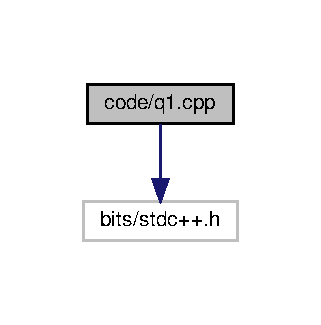
\includegraphics[width=286pt]{q1_8cpp__incl}
\end{center}
\end{figure}
\subsection*{Classes}
\begin{DoxyCompactItemize}
\item 
struct \hyperlink{struct_r_b_t_node}{R\+B\+T\+Node}
\begin{DoxyCompactList}\small\item\em \hyperlink{struct_r_b_t_node}{R\+B\+T\+Node} for red black tree. \end{DoxyCompactList}\item 
class \hyperlink{class_r_b_tree}{R\+B\+Tree}
\begin{DoxyCompactList}\small\item\em Class to represent Red-\/\+Black Tree. \end{DoxyCompactList}\item 
class \hyperlink{class_node}{Node}
\item 
class \hyperlink{class_a_v_l_tree}{A\+V\+L\+Tree}
\begin{DoxyCompactList}\small\item\em Class for A\+VL Tree. \end{DoxyCompactList}\item 
struct \hyperlink{structnode}{node}
\end{DoxyCompactItemize}
\subsection*{Enumerations}
\begin{DoxyCompactItemize}
\item 
enum \hyperlink{q1_8cpp_ab87bacfdad76e61b9412d7124be44c1c}{Color} \{ \hyperlink{q1_8cpp_ab87bacfdad76e61b9412d7124be44c1caf80f9a890089d211842d59625e561f88}{R\+ED}, 
\hyperlink{q1_8cpp_ab87bacfdad76e61b9412d7124be44c1caf77fb67151d0c18d397069ad8c271ba3}{B\+L\+A\+CK}
 \}
\end{DoxyCompactItemize}
\subsection*{Functions}
\begin{DoxyCompactItemize}
\item 
struct \hyperlink{structnode}{node} $\ast$ \hyperlink{q1_8cpp_a8a3ee315f73c586e51fcd202c4cd8662}{new\+Node} (int item)
\item 
void \hyperlink{q1_8cpp_a8e025ab1257df618068309e6a30fc93a}{inorder} (struct \hyperlink{structnode}{node} $\ast$root)
\item 
struct \hyperlink{structnode}{node} $\ast$ \hyperlink{q1_8cpp_a20a3b180a7700373071305e18971bb5e}{insert} (struct \hyperlink{structnode}{node} $\ast$\hyperlink{structnode}{node}, int key)
\item 
void \hyperlink{q1_8cpp_aa42e420e039d99993459c8d8a4fbdbdb}{print\+Path} (\hyperlink{structnode}{node} $\ast$rt, string s)
\item 
void \hyperlink{q1_8cpp_acfc11a0afabf3a77687b4b156d69cdd5}{get\+All\+Paths} (struct \hyperlink{structnode}{node} $\ast$\hyperlink{q1_8cpp_aab7df7514eae49d8d3b271504678bc75}{B\+ST})
\item 
void \hyperlink{q1_8cpp_a46640f831c90fba2fb20af78cea58a0c}{level\+Vise\+Indentation\+Helper} (\hyperlink{structnode}{node} $\ast$rt, int l)
\item 
void \hyperlink{q1_8cpp_a6e841fa6644d2916b88392bfcf8376d1}{level\+Vise\+Indentation} (\hyperlink{structnode}{node} $\ast$root)
\item 
void \hyperlink{q1_8cpp_aee650708cb84556644f8a4f6e7611c06}{create\+A\+V\+L\+Tree} (struct \hyperlink{structnode}{node} $\ast$rt)
\item 
int \hyperlink{q1_8cpp_ae66f6b31b5ad750f1fe042a706a4e3d4}{main} ()
\end{DoxyCompactItemize}
\subsection*{Variables}
\begin{DoxyCompactItemize}
\item 
\hyperlink{class_a_v_l_tree}{A\+V\+L\+Tree} \hyperlink{q1_8cpp_afa690420f01f46758f4ecfd9088af2b1}{A\+VL}
\item 
struct \hyperlink{structnode}{node} $\ast$ \hyperlink{q1_8cpp_aab7df7514eae49d8d3b271504678bc75}{B\+ST} = N\+U\+LL
\end{DoxyCompactItemize}


\subsection{Enumeration Type Documentation}
\mbox{\Hypertarget{q1_8cpp_ab87bacfdad76e61b9412d7124be44c1c}\label{q1_8cpp_ab87bacfdad76e61b9412d7124be44c1c}} 
\index{q1.\+cpp@{q1.\+cpp}!Color@{Color}}
\index{Color@{Color}!q1.\+cpp@{q1.\+cpp}}
\subsubsection{\texorpdfstring{Color}{Color}}
{\footnotesize\ttfamily enum \hyperlink{q1_8cpp_ab87bacfdad76e61b9412d7124be44c1c}{Color}}

\begin{DoxyEnumFields}{Enumerator}
\raisebox{\heightof{T}}[0pt][0pt]{\index{R\+ED@{R\+ED}!q1.\+cpp@{q1.\+cpp}}\index{q1.\+cpp@{q1.\+cpp}!R\+ED@{R\+ED}}}\mbox{\Hypertarget{q1_8cpp_ab87bacfdad76e61b9412d7124be44c1caf80f9a890089d211842d59625e561f88}\label{q1_8cpp_ab87bacfdad76e61b9412d7124be44c1caf80f9a890089d211842d59625e561f88}} 
R\+ED&\\
\hline

\raisebox{\heightof{T}}[0pt][0pt]{\index{B\+L\+A\+CK@{B\+L\+A\+CK}!q1.\+cpp@{q1.\+cpp}}\index{q1.\+cpp@{q1.\+cpp}!B\+L\+A\+CK@{B\+L\+A\+CK}}}\mbox{\Hypertarget{q1_8cpp_ab87bacfdad76e61b9412d7124be44c1caf77fb67151d0c18d397069ad8c271ba3}\label{q1_8cpp_ab87bacfdad76e61b9412d7124be44c1caf77fb67151d0c18d397069ad8c271ba3}} 
B\+L\+A\+CK&\\
\hline

\end{DoxyEnumFields}


Definition at line 6 of file q1.\+cpp.



\subsection{Function Documentation}
\mbox{\Hypertarget{q1_8cpp_aee650708cb84556644f8a4f6e7611c06}\label{q1_8cpp_aee650708cb84556644f8a4f6e7611c06}} 
\index{q1.\+cpp@{q1.\+cpp}!create\+A\+V\+L\+Tree@{create\+A\+V\+L\+Tree}}
\index{create\+A\+V\+L\+Tree@{create\+A\+V\+L\+Tree}!q1.\+cpp@{q1.\+cpp}}
\subsubsection{\texorpdfstring{create\+A\+V\+L\+Tree()}{createAVLTree()}}
{\footnotesize\ttfamily void create\+A\+V\+L\+Tree (\begin{DoxyParamCaption}\item[{struct \hyperlink{structnode}{node} $\ast$}]{rt }\end{DoxyParamCaption})}

This method will be used to create A\+VL Tree from in\+Order traversal of Binary Search Tree. 
\begin{DoxyParams}{Parameters}
{\em rt} & Root of the binary search tree(\+B\+S\+T). \\
\hline
\end{DoxyParams}
\begin{DoxyAuthor}{Author}
Kavya Barnwal 
\end{DoxyAuthor}
\begin{DoxyDate}{Date}
20/08/2019 
\end{DoxyDate}


Definition at line 770 of file q1.\+cpp.

\mbox{\Hypertarget{q1_8cpp_acfc11a0afabf3a77687b4b156d69cdd5}\label{q1_8cpp_acfc11a0afabf3a77687b4b156d69cdd5}} 
\index{q1.\+cpp@{q1.\+cpp}!get\+All\+Paths@{get\+All\+Paths}}
\index{get\+All\+Paths@{get\+All\+Paths}!q1.\+cpp@{q1.\+cpp}}
\subsubsection{\texorpdfstring{get\+All\+Paths()}{getAllPaths()}}
{\footnotesize\ttfamily void get\+All\+Paths (\begin{DoxyParamCaption}\item[{struct \hyperlink{structnode}{node} $\ast$}]{B\+ST }\end{DoxyParamCaption})}

This method will be used to print all the paths from root node to the N\+U\+LL pointers. 
\begin{DoxyParams}{Parameters}
{\em B\+ST} & Root of B\+ST. \\
\hline
\end{DoxyParams}
\begin{DoxyAuthor}{Author}
Kavya Barnwal 
\end{DoxyAuthor}
\begin{DoxyDate}{Date}
20/08/2019 
\end{DoxyDate}


Definition at line 721 of file q1.\+cpp.

\mbox{\Hypertarget{q1_8cpp_a8e025ab1257df618068309e6a30fc93a}\label{q1_8cpp_a8e025ab1257df618068309e6a30fc93a}} 
\index{q1.\+cpp@{q1.\+cpp}!inorder@{inorder}}
\index{inorder@{inorder}!q1.\+cpp@{q1.\+cpp}}
\subsubsection{\texorpdfstring{inorder()}{inorder()}}
{\footnotesize\ttfamily void inorder (\begin{DoxyParamCaption}\item[{struct \hyperlink{structnode}{node} $\ast$}]{root }\end{DoxyParamCaption})}

A utility function to do inorder traversal of B\+ST. 
\begin{DoxyParams}{Parameters}
{\em node} & Root of B\+ST. \\
\hline
{\em key} & data to be inserted. \\
\hline
\end{DoxyParams}
\begin{DoxyAuthor}{Author}
Kavya Barnwal 
\end{DoxyAuthor}
\begin{DoxyDate}{Date}
20/08/2019 
\end{DoxyDate}


Definition at line 659 of file q1.\+cpp.

\mbox{\Hypertarget{q1_8cpp_a20a3b180a7700373071305e18971bb5e}\label{q1_8cpp_a20a3b180a7700373071305e18971bb5e}} 
\index{q1.\+cpp@{q1.\+cpp}!insert@{insert}}
\index{insert@{insert}!q1.\+cpp@{q1.\+cpp}}
\subsubsection{\texorpdfstring{insert()}{insert()}}
{\footnotesize\ttfamily struct \hyperlink{structnode}{node}$\ast$ insert (\begin{DoxyParamCaption}\item[{struct \hyperlink{structnode}{node} $\ast$}]{node,  }\item[{int}]{key }\end{DoxyParamCaption})}

A utility function to insert a new node with given key in B\+ST. 
\begin{DoxyParams}{Parameters}
{\em node} & Root of B\+ST. \\
\hline
{\em key} & data to be inserted. \\
\hline
\end{DoxyParams}
\begin{DoxyAuthor}{Author}
Kavya Barnwal 
\end{DoxyAuthor}
\begin{DoxyDate}{Date}
20/08/2019 
\end{DoxyDate}


Definition at line 676 of file q1.\+cpp.

\mbox{\Hypertarget{q1_8cpp_a6e841fa6644d2916b88392bfcf8376d1}\label{q1_8cpp_a6e841fa6644d2916b88392bfcf8376d1}} 
\index{q1.\+cpp@{q1.\+cpp}!level\+Vise\+Indentation@{level\+Vise\+Indentation}}
\index{level\+Vise\+Indentation@{level\+Vise\+Indentation}!q1.\+cpp@{q1.\+cpp}}
\subsubsection{\texorpdfstring{level\+Vise\+Indentation()}{levelViseIndentation()}}
{\footnotesize\ttfamily void level\+Vise\+Indentation (\begin{DoxyParamCaption}\item[{\hyperlink{structnode}{node} $\ast$}]{root }\end{DoxyParamCaption})}

This method will be used to print the Binary Search Tree(\+B\+S\+T) with lavel-\/wise-\/indentation. 
\begin{DoxyParams}{Parameters}
{\em root} & Root of B\+ST. \\
\hline
\end{DoxyParams}
\begin{DoxyAuthor}{Author}
Kavya Barnwal 
\end{DoxyAuthor}
\begin{DoxyDate}{Date}
20/08/2019 
\end{DoxyDate}


Definition at line 759 of file q1.\+cpp.

\mbox{\Hypertarget{q1_8cpp_a46640f831c90fba2fb20af78cea58a0c}\label{q1_8cpp_a46640f831c90fba2fb20af78cea58a0c}} 
\index{q1.\+cpp@{q1.\+cpp}!level\+Vise\+Indentation\+Helper@{level\+Vise\+Indentation\+Helper}}
\index{level\+Vise\+Indentation\+Helper@{level\+Vise\+Indentation\+Helper}!q1.\+cpp@{q1.\+cpp}}
\subsubsection{\texorpdfstring{level\+Vise\+Indentation\+Helper()}{levelViseIndentationHelper()}}
{\footnotesize\ttfamily void level\+Vise\+Indentation\+Helper (\begin{DoxyParamCaption}\item[{\hyperlink{structnode}{node} $\ast$}]{rt,  }\item[{int}]{l }\end{DoxyParamCaption})}

Helper method for method \hyperlink{q1_8cpp_a6e841fa6644d2916b88392bfcf8376d1}{level\+Vise\+Indentation()}. 
\begin{DoxyParams}{Parameters}
{\em root} & Root of B\+ST. \\
\hline
{\em l} & level of that node. \\
\hline
\end{DoxyParams}
\begin{DoxyAuthor}{Author}
Kavya Barnwal 
\end{DoxyAuthor}
\begin{DoxyDate}{Date}
20/08/2019 
\end{DoxyDate}


Definition at line 738 of file q1.\+cpp.

\mbox{\Hypertarget{q1_8cpp_ae66f6b31b5ad750f1fe042a706a4e3d4}\label{q1_8cpp_ae66f6b31b5ad750f1fe042a706a4e3d4}} 
\index{q1.\+cpp@{q1.\+cpp}!main@{main}}
\index{main@{main}!q1.\+cpp@{q1.\+cpp}}
\subsubsection{\texorpdfstring{main()}{main()}}
{\footnotesize\ttfamily int main (\begin{DoxyParamCaption}{ }\end{DoxyParamCaption})}



Definition at line 781 of file q1.\+cpp.

\mbox{\Hypertarget{q1_8cpp_a8a3ee315f73c586e51fcd202c4cd8662}\label{q1_8cpp_a8a3ee315f73c586e51fcd202c4cd8662}} 
\index{q1.\+cpp@{q1.\+cpp}!new\+Node@{new\+Node}}
\index{new\+Node@{new\+Node}!q1.\+cpp@{q1.\+cpp}}
\subsubsection{\texorpdfstring{new\+Node()}{newNode()}}
{\footnotesize\ttfamily struct \hyperlink{structnode}{node}$\ast$ new\+Node (\begin{DoxyParamCaption}\item[{int}]{item }\end{DoxyParamCaption})}

A utility function to create a new B\+ST node. 
\begin{DoxyParams}{Parameters}
{\em item} & data to be inserted. \\
\hline
\end{DoxyParams}
\begin{DoxyAuthor}{Author}
Kavya Barnwal 
\end{DoxyAuthor}
\begin{DoxyDate}{Date}
20/08/2019 
\end{DoxyDate}


Definition at line 644 of file q1.\+cpp.

\mbox{\Hypertarget{q1_8cpp_aa42e420e039d99993459c8d8a4fbdbdb}\label{q1_8cpp_aa42e420e039d99993459c8d8a4fbdbdb}} 
\index{q1.\+cpp@{q1.\+cpp}!print\+Path@{print\+Path}}
\index{print\+Path@{print\+Path}!q1.\+cpp@{q1.\+cpp}}
\subsubsection{\texorpdfstring{print\+Path()}{printPath()}}
{\footnotesize\ttfamily void print\+Path (\begin{DoxyParamCaption}\item[{\hyperlink{structnode}{node} $\ast$}]{rt,  }\item[{string}]{s }\end{DoxyParamCaption})}

Helper method for method \hyperlink{q1_8cpp_acfc11a0afabf3a77687b4b156d69cdd5}{get\+All\+Paths()}. 
\begin{DoxyParams}{Parameters}
{\em rt} & Root of B\+ST. \\
\hline
{\em s} & string containing details of nodes traversed. \\
\hline
\end{DoxyParams}
\begin{DoxyAuthor}{Author}
Kavya Barnwal 
\end{DoxyAuthor}
\begin{DoxyDate}{Date}
20/08/2019 
\end{DoxyDate}


Definition at line 699 of file q1.\+cpp.



\subsection{Variable Documentation}
\mbox{\Hypertarget{q1_8cpp_afa690420f01f46758f4ecfd9088af2b1}\label{q1_8cpp_afa690420f01f46758f4ecfd9088af2b1}} 
\index{q1.\+cpp@{q1.\+cpp}!A\+VL@{A\+VL}}
\index{A\+VL@{A\+VL}!q1.\+cpp@{q1.\+cpp}}
\subsubsection{\texorpdfstring{A\+VL}{AVL}}
{\footnotesize\ttfamily \hyperlink{class_a_v_l_tree}{A\+V\+L\+Tree} A\+VL}



Definition at line 628 of file q1.\+cpp.

\mbox{\Hypertarget{q1_8cpp_aab7df7514eae49d8d3b271504678bc75}\label{q1_8cpp_aab7df7514eae49d8d3b271504678bc75}} 
\index{q1.\+cpp@{q1.\+cpp}!B\+ST@{B\+ST}}
\index{B\+ST@{B\+ST}!q1.\+cpp@{q1.\+cpp}}
\subsubsection{\texorpdfstring{B\+ST}{BST}}
{\footnotesize\ttfamily struct \hyperlink{structnode}{node}$\ast$ B\+ST = N\+U\+LL}



Definition at line 636 of file q1.\+cpp.


%--- End generated contents ---

% Index
\backmatter
\newpage
\phantomsection
\clearemptydoublepage
\addcontentsline{toc}{chapter}{Index}
\printindex

\end{document}
